\documentclass{article}

% if you need to pass options to natbib, use, e.g.:
%     \PassOptionsToPackage{numbers, compress}{natbib}
% before loading neurips_2019

% ready for submission
% \usepackage{neurips_2019}

% to compile a preprint version, e.g., for submission to arXiv, add add the
% [preprint] option:
%     \usepackage[preprint]{neurips_2019}

% to compile a camera-ready version, add the [final] option, e.g.:
     \usepackage[final]{mlcb_2019}

% to avoid loading the natbib package, add option nonatbib:
%     \usepackage[nonatbib]{neurips_2019}

\usepackage[utf8]{inputenc} % allow utf-8 input
\usepackage[T1]{fontenc}    % use 8-bit T1 fonts
\usepackage{hyperref}       % hyperlinks
\usepackage{url}            % simple URL typesetting
\usepackage{booktabs}       % professional-quality tables
\usepackage{amsfonts}       % blackboard math symbols
\usepackage{nicefrac}       % compact symbols for 1/2, etc.
\usepackage{microtype}
\usepackage{amsmath}      % microtypography
\usepackage{bm}
\usepackage{graphicx}
\usepackage{verbatim}
\usepackage{wrapfig}
\usepackage[font=small]{caption}
\usepackage{enumitem}
\usepackage{amsmath}
%\usepackage{floatrow}

%\addtolength{\belowcaptionskip}{-20pt}

\title{End-to-end RNA Secondary Structure Prediction using Autoregressive Deep Convolutional Neural Network}

% The \author macro works with any number of authors. There are two commands
% used to separate the names and addresses of multiple authors: \And and \AND.
%
% Using \And between authors leaves it to LaTeX to determine where to break the
% lines. Using \AND forces a line break at that point. So, if LaTeX puts 3 of 4
% authors names on the first line, and the last on the second line, try using
% \AND instead of \And before the third author name.

% double-blind
%\author{%
%  TODO \\
%  Department of Electrical and Computer Engineering\\
%  University of Toronto\\
%  \texttt{todo@toronto.edu} \\
%  % examples of more authors
%  % \And
%  % Coauthor \\
%  % Affiliation \\
%  % Address \\
%  % \texttt{email} \\
%  % \AND
%  % Coauthor \\
%  % Affiliation \\
%  % Address \\
%  % \texttt{email} \\
%  % \And
%  % Coauthor \\
%  % Affiliation \\
%  % Address \\
%  % \texttt{email} \\
%  % \And
%  % Coauthor \\
%  % Affiliation \\
%  % Address \\
%  % \texttt{email} \\
%}

\begin{document}

\maketitle

%\begin{abstract}
%  TODO
%\end{abstract}

\vspace*{-7em}

\section{Introduction}

%Once believed to be an intermediate molecule that serves as a messenger between DNA and protein,
%RNA is now known to be involved in many aspects in gene regulation and expression.
Unlike DNA which typically forms stable double helix between two molecules, RNA is highly flexible
so a single RNA molecule can fold onto itself by
forming base pairs via hydrogen bond, including Watson-Crick pairs A-U,
G-C and non-canonical pairs such as G-U.
Base pairs form local structures like stems and loops,
which assemble into the global secondary structure.
%These base pairs act as building blocks, from which local structure forms? global?

State-of-the-art RNA secondary structure prediction algorithms
like ViennaRNA\cite{lorenz2011viennarna} and Mfold\cite{zuker2003mfold}
are based on thermodynamics.
Free energy of each type of local structure is measured experimentally,
and total free energy is assumed to be the sum of local energy terms,
which is minimized efficiently via dynamic programming (DP).
Although researchers have worked out a large set of local structure types and
their associated formulation for free energy calculation,
there is no guarantee that it is accurate and complete.
There have been efforts to fine-tune the free energy parameters by
training on experimentally solved structures\cite{andronescu2007efficient},
but it is still limited by the known set of local structure types.
Another limitation of DP-based approaches is that
it is incapable of predicting nested base pairs that appear in structures such as pseudoknot.


%Moreover, over the last decade,
%combination of RNA structure probing and high throughput sequencing has enabled
%the measurement of genome-wide RNA structural at single nucleotide resolution in multiple organisms and cell types,
%which have only been combined? with dynamic programming using heuristics (ref?).
%Such data also exhibit a high level of noise and sometimes with missing data (ref, sequencing, DMS),
%which also calls for new approaches that can be trained end-to-end on different types of data,
%to model ?differences in cell types and conditions.

On the other hand, over the last decade,
a combination of RNA structure probing and high-throughput sequencing has enabled
the measurement of genome-wide RNA structures at single nucleotide resolution in
multiple organisms and cell types\cite{mortimer2014insights, bevilacqua2016genome}.
Due to the level of noise and missing data present in high-throughput experiments,
a more flexible modeling approach is needed which can be trained on different types of data.
%Such data can be valuable in learning cell type specific RNA secondary structure model,
%
%Such data also exhibit a high level of noise and sometimes with missing data (ref, sequencing, DMS),
%which also calls for new approaches that can be trained end-to-end on different types of data,
%to model ?differences in cell types and conditions.

In this work, we propose a autoregressive deep convolutional neural network that can be trained end-to-end on
sequences and structures. Given an input RNA sequence,
the model can generate a distribution of structures, including ones with pseudoknot.
%We start by describing the problem formulation, followed by a brief review of
%related work, and present the model
%differentiable

%TODO if we mention the above we'll need to talk about how to train on those data.
%
%sequence alone
%
%one sequence, many structures

\begin{wrapfigure}{R}
        \centering
        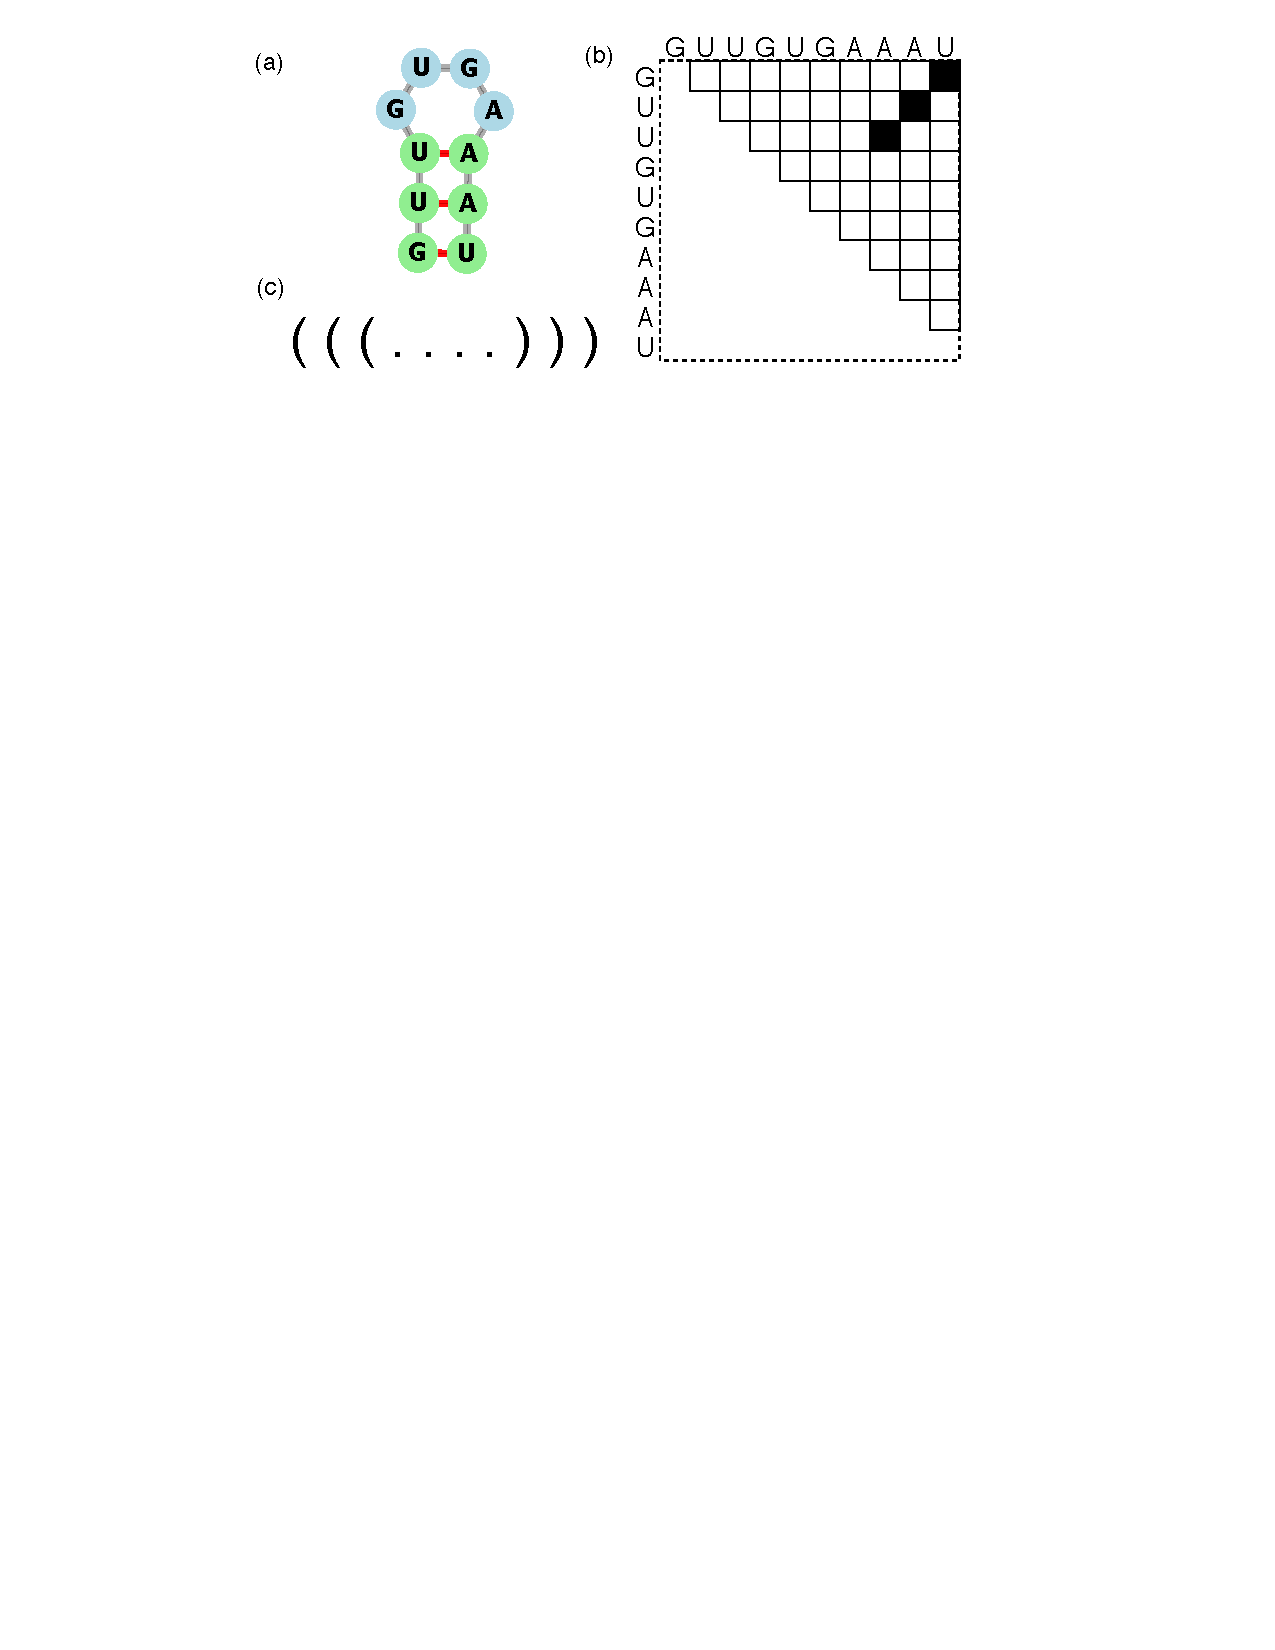
\includegraphics[width=0.3\textwidth]{plot/rna_ss_binary_mat.pdf}
        \caption{Three different ways to represent secondary structure. (a) undirected graph, generated by \cite{kerpedjiev2015forna}, (b) upper triangular binary matrix, (c) dot-bracket notation.}
        \label{fig:rna_ss_binary_mat}
        \centering
\end{wrapfigure}

\subsection{Problem formulation}

Given an RNA sequence of length $L$, we are interested in all possible secondary structures.
%There are three common ways to represent a specific RNA secondary structure:
To represent a specific secondary structure, there are three commonly used conventions:
(1) undirected graph, where each node is a base in the sequence, and each edge represents base pairing.
(2) upper triangular matrix (excluding the diagonal)
of size $L \times L$ with binary values, where a value of $1$ at $(i, j)$ represents
base pairing between sequence position $i$ and $j$, and $0$ represents no base paring.
(3) dot-bracket notation of length $L$ where unpaired bases are denoted as dots,
    and paired bases are represented as left and right brackets.
%When pseudoknot is present, different styles of bracket needs to be used to represent nested structures.


%\begin{itemize}
%
%    \item Undirected graph, where each node is a base in the sequence, and each vertex represent base pairing.
%
%    \item Upper triangular matrix (excluding the diagonal)
%of size $L \times L$ with binary values, where a value of $1$ at $(i, j)$ represents
%base pairing between sequence position $i$ and $j$, and $0$ represents no base paring.
%
%    \item A dot-bracket notation of length $L$ where unpaired based are denoted as dots,
%    and paired bases are represented as left and right brackets.
%
%\end{itemize}

As an example, for a short RNA sequence GUUGUGAAAU, one possible structure it can take on
%(Entry \verb|CRW_00083| from \cite{andronescu2008rna})   # TODO this entry nmumber is not correct!
%takes a structure that
consists of a stem and a loop, as seen in Fig \ref{fig:rna_ss_binary_mat}(a), represented by an undirected graph.
Such structure can also be represented by a $10 \times 10$ upper triangular matrix with all $0$'s,
except for positions
%$y_{1, 10}, y_{2, 9}$ and $y_{3, 8}$,
$(1, 10), (2, 9)$ and $(3, 8)$,
all being $1$, as shown in Fig \ref{fig:rna_ss_binary_mat}(b).
This contiguous stretch of $1$'s along the diagonal corresponds to the stem formed by the three base pairs: G-U, U-A and U-A.
The equivalent dot-bracket notation is shown in Fig \ref{fig:rna_ss_binary_mat}(c), where the stem is represented
by three pairs of left-right brackets.
%(TODO define x and y first)




%\begin{wrapfigure}{R}
%%    \begin{figure}[h]
%        \centering
%        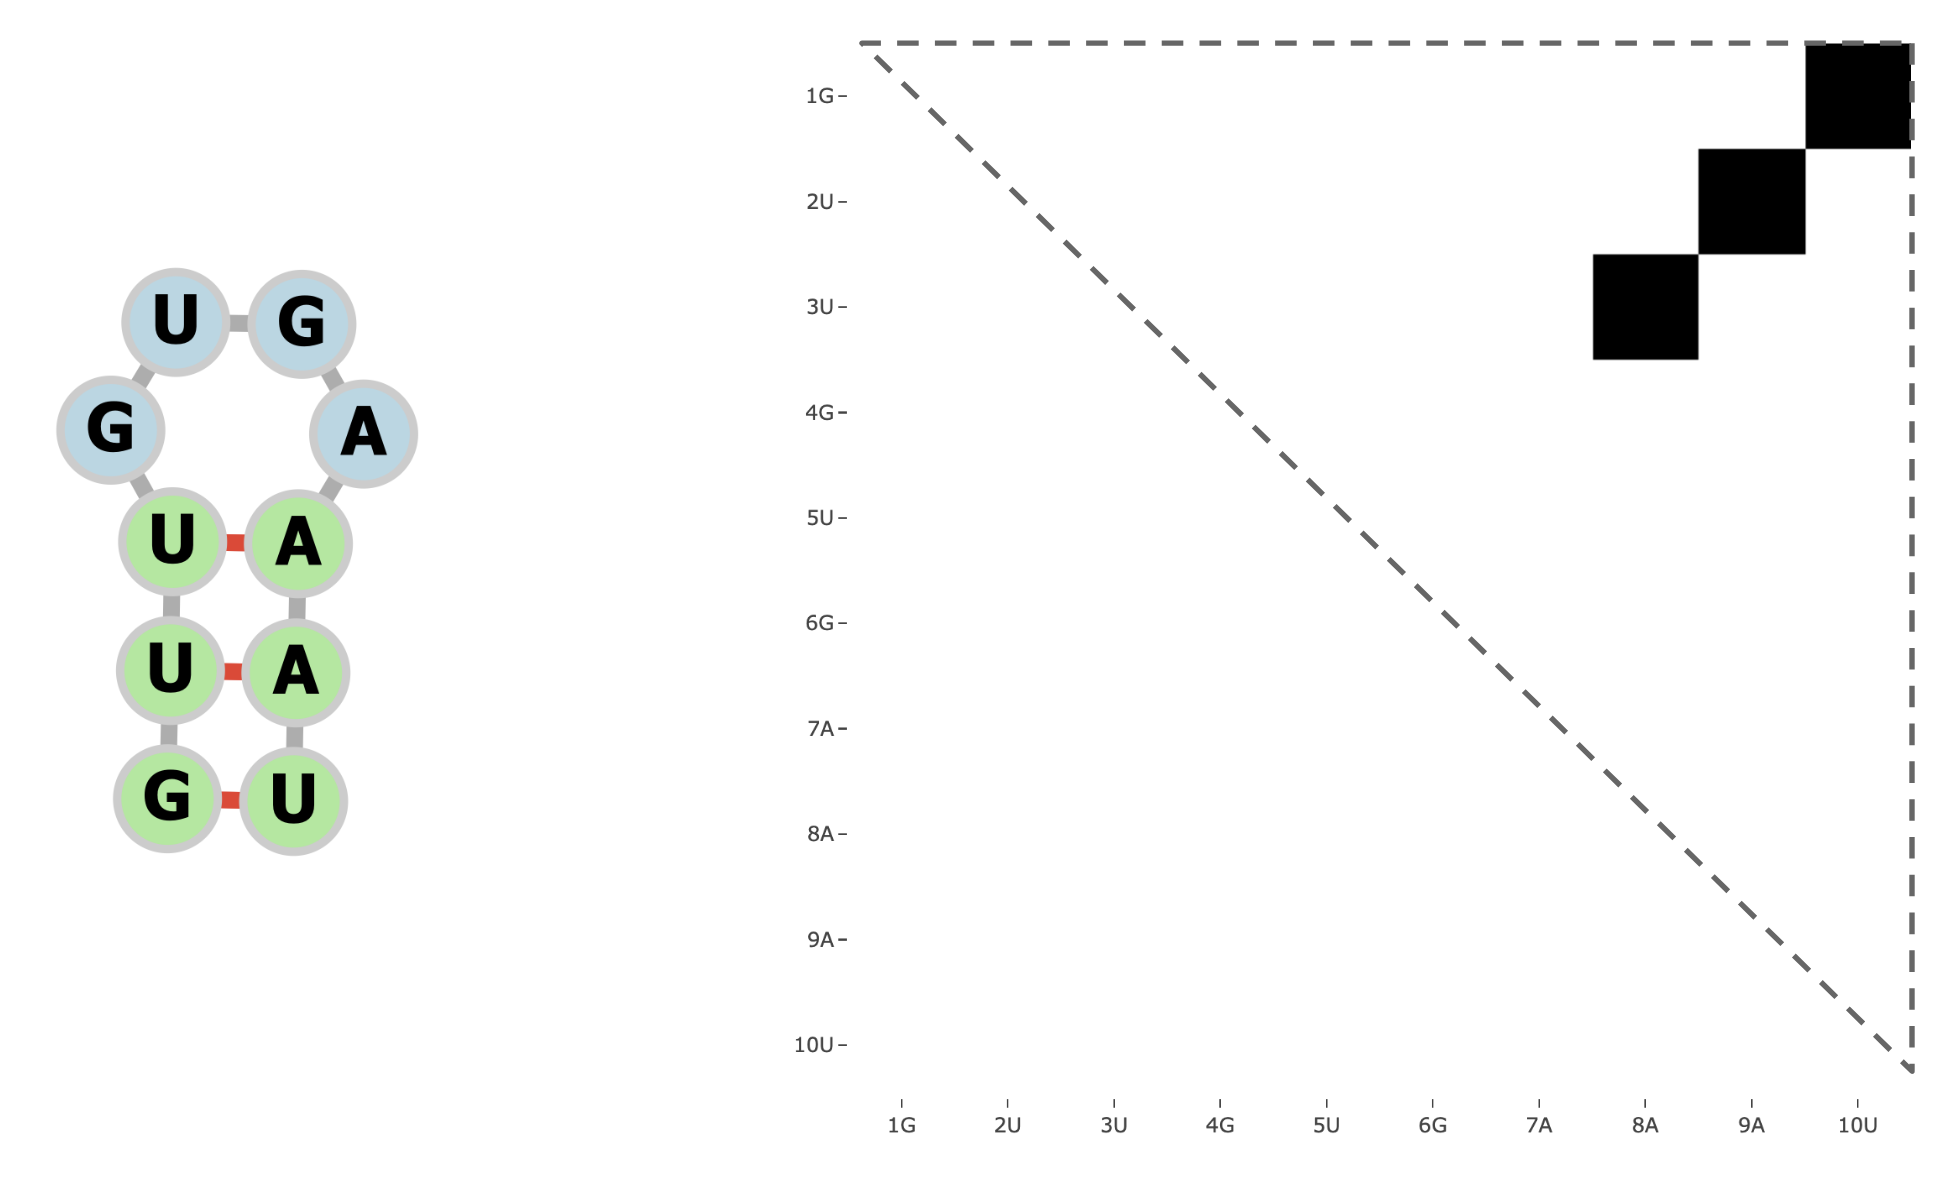
\includegraphics[width=0.5\textwidth]{plot/rna_ss_binary_mat.png}
%        \caption{TODO}
%        \label{fig:rna_ss_binary_mat}
%        \centering
%%    \end{figure}
%\end{wrapfigure}



%TODO maybe talk about pairing matrix and dot-bracket notation here, to make it easier for literature review.

\begin{wrapfigure}{R}
    \centering
    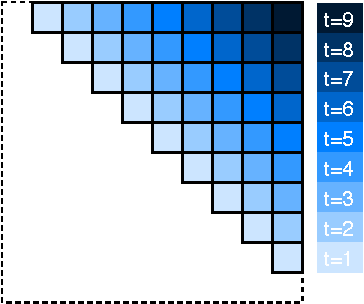
\includegraphics[width=0.18\textwidth]{plot/autoregressive_direction.pdf}
    \caption{Generative process implied by Equation \ref{eq:conditional_distribution}.}
    \label{fig:autoregressive_direction}
    \centering
\end{wrapfigure}

\subsection{Related work}

%There have been a few work that solve partial problem.... % TODO ??
%Several work exist that applies neural network in
Several groups have tried to apply neural network in modeling RNA secondary structure.
To the best of our knowledge, existing work either solves a partial problem,
or attempts at modeling the problem end-to-end,
but requires complicated post-processing to yield valid structure prediction.

Wu\cite{wu2018convolutional} presented a convolution neural network to predict the free energy of local structure motifs.
%Convolution was run on circular matrix representation of the structure motif, to reflect the loop-like nature of local structures.
%Circular convolution was proposed as a nature fit for loop-like structures.
%The model was trained on experimentally measured free energy of short structure motifs,
%as well as random structure motifs whose energy was estimated using existing linear approximation models.
Although it shows promising results on modeling the free energy of short structure motif from experimental data
and on estimating the free energy for a \textit{given} structure,
it does not solve the problem of predicting structure from sequence.

%Other work were done to tackle the learning problem end-to-end.
Researchers have also framed the problem as a sequence-to-sequence learning task.
The proposed models either predict the pairing probability for each base,
or some forms of the dot-bracket notation.
Willmott et. al\cite{willmottstate} proposed a bidirectional LSTM that predicts
the per-position probability for 3 classes: paired, unpaired, and end-of-sequence.
The model was trained on sequences that belong to the same RNA family,
so it is unclear whether the model generalizes to other types of RNAs.
Zhang et. al\cite{zhang2019new} proposed a convolutional neural network to predict
the dot-bracket notation, where each position is encoded as a 3-class softmax: left bracket, right bracket and dot.
In order for a dot-bracket notation to yield valid structure, it has to follow a few syntactic constraints.
For example, each left bracket needs to have a corresponding right bracket.
As the authors mentioned in the paper, output produced by the neural network
was not guaranteed to be valid, thus needed to be further processed by dynamic programming
to yield a valid structure prediction.
Wang et. al\cite{wang2019dmfold} used bidirectional LSTM to predict the dot-bracket notation as a
7-class softmax, which includes additional bracket notations to allow for pseudoknot.
Similar to \cite{zhang2019new}, the prediction did not yield a
valid structure, and needed further post-processing.
Furthermore, they used a dataset of only four RNA families,
but reported performance based on randomized training and validation set split.
Since there is high level of sequence similarity within the same family,
generalization performance of the model remains unclear.
%Random split is almost certain to result in sequences from the same family to be in both the training and validation set,
%thus the generalization performance of the model remains unclear.
%he model was trained on only ? RNA families, and CV split was random,
%so generalization performance is unclear.



%Existing work either solves a partial problem, or attempts at modelling the problem end-to-end,
%but requires complicated post-processing to yield valid structure prediction.
%In this work, we propose a novel method to model the sequence to structure predictive task end-to-end, with
%no additional post-processing.



%RNA Secondary Structure Prediction by MFT Neural Networks
%\cite{apolloni2003rna}

%A New Method of RNA Secondary Structure Prediction Based on Convolutional Neural Network and Dynamic Programming
%\cite{zhang2019new}

%Convolutional models of RNA energetics
%\cite{wu2018convolutional}

%Recurrent Neural Networks and Their Applications to RNA Secondary Structure Inference
%\cite{willmott2018recurrent}

%RNA Secondary Structure Prediction Using Neural Machine Translation
%\cite{zhang2016rna}

%State inference of RNA secondary structures with deep recurrent neural networks  (replace above thesis)
%\cite{willmottstate}

%SCFG: Learning RNA secondary structure (only) from structure probing data
%not that relevant, maybe we can skip it
%
%TODO talk about what's lacking in all above approaches.


%\begin{itemize}
%
%    \item State-of-the-art methods based on dynamic programming.
%Basic building blocks are known local structure, with their associated free energy measured experimentally.
%Fixed energy parameters and hand-crafted rules.
%
%    \item Emerging new dataset calls for flexible, extensible,
%    end-to-end model that can be trained on new types of dataset (noisy, missing value).
%
%    \item TODO review other papers using NN and discuss what's lacking.
%
%\end{itemize}

%notation: we use ??? to represent a binary upper triangular matrix of size LxL.


\begin{wrapfigure}{R}
%    \begin{figure}[h]
        \centering
        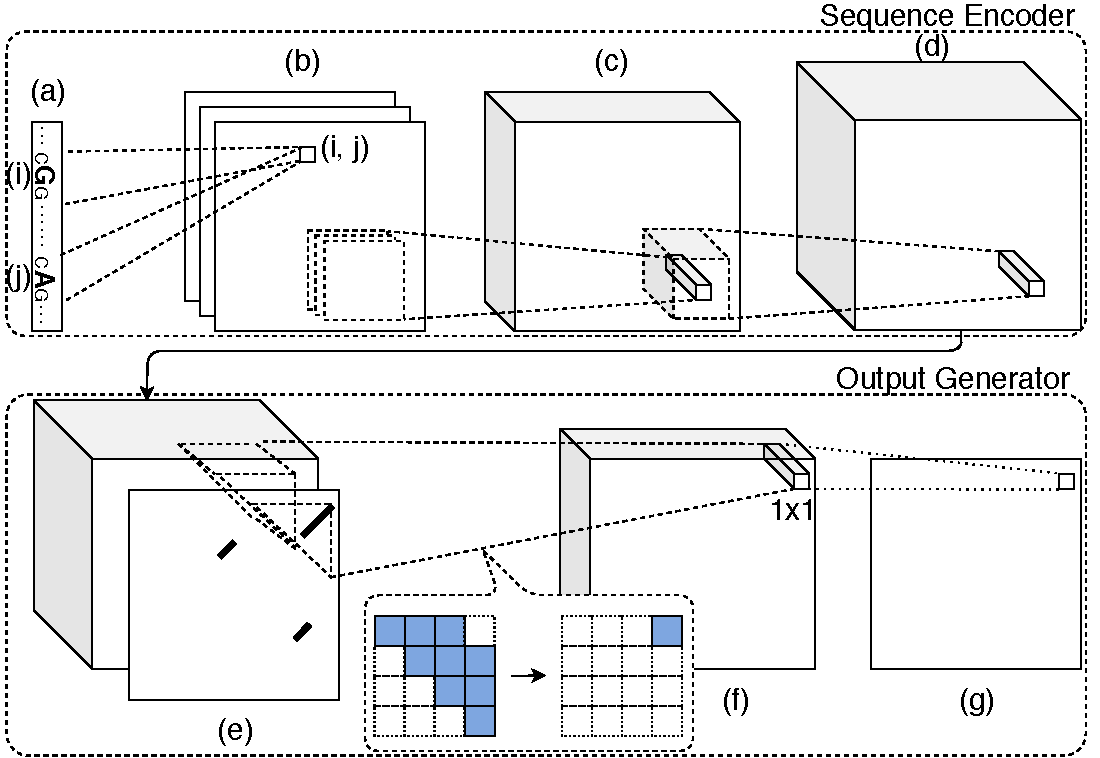
\includegraphics[width=0.5\textwidth]{plot/nn_arch_1.pdf}
        \caption{Proposed model architecture. Top: sequence encoder. Bottom: output generator.}
        \vspace{-8em}
        \label{fig:nn_arch_1}
        \centering
%    \end{figure}
\end{wrapfigure}



\section{Method}


In this work, we propose a autoregressive deep convolutional neural network that is trained end-to-end on
dataset with sequences and structures.
The model is capable of generating a distribution of structures conditioned on the input sequence,
including structures with pseudoknot.



We formulate the predictive task as a conditional generative process.
Specifically, given an input sequence of length $L$: $\bm{x} = (x_1, x_2, \dots x_{L})$,
we want to predict a distribution of structures conditioned on the sequence $P(\bm{Y} \mid \bm{x})$,
where the structure $\bm{Y}$ is represented by an upper triangular matrix of size $L \times L$, as defined in Fig \ref{fig:rna_ss_binary_mat}(b).

%(TODO use the above notation).

%(move the following paragraph to the model section)
We factorize the conditional distribution as follows:
%In this work, we pick a specific way to factorize the conditional distribution,

%\begin{equation} \label{eq:conditional_distribution}
%{\scriptstyle
%P(\bm{Y} \mid \bm{x}) = P(\{y_{i, i+1}\}_{i=1, 2, \dots L-1} \mid \bm{x})
%P(\{y_{i, i+2}\}_{i=1, 2, \dots L-2} \mid \bm{x}, \{y_{i, i+1}\}_{i=1, 2, \dots L-1})
%\dots
%P(y_{1, L} \mid \bm{x}, \{y_{i, j}\}^{i \neq 1}_{j \neq L})}
%\end{equation}


\begin{equation}
    \label{eq:conditional_distribution}
    \begin{split}
        P(\bm{Y} \mid \bm{x}) =& P(\{y_{i, i+1}\}_{i=1, \dots L-1} \mid \bm{x}) \\
        & P(\{y_{i, i+2}\}_{i=1, \dots L-2} \mid \bm{x}, \{y_{i, i+1}\}_{i=1, \dots L-1}) \\
        & \dots \\
        & P(y_{1, L} \mid \bm{x}, \{y_{i, j}\}^{i \neq 1}_{j \neq L})
    \end{split}
\end{equation}

%which mimcs the autoregressive process, where the time axis in our case is the distance to the off-diagonal line.

The generative process implied by such formulation is illustrated in Fig \ref{fig:autoregressive_direction}.
Starting from the slice adjacent to the off-diagonal line (light blue with $t=1$),
we generate one off-diagonal slice at a time, conditioned on the input sequence and the previous slices.
%We generate one off-diagonal slice at a time, conditioned on the input sequence and the previous slices,
%starting from the one adjacent to the off-diagonal line, shown in light blue with $t=1$.
This process continues until we fill the upper triangular matrix,
where the last entry (dark blue, with $t=9$) is conditioned on the input and the entire upper triangular matrix except for itself.
Intuitively, the distance to the off-diagonal line is analogous to the ``timestamp'' as in classic autoregressive models.

%TODO re-generate plot using draw.io, or use the model plot?
%
%We generate one off diagonal slice at a time, conditioned on the input sequence and the previous slices,
%starting from the one adjacent to the diagonal line, as shown in yellow on the plot.
%When generating the second slice (in green), we condition on the input sequence and the generated values in the first slice (in yellow).
%When generating the third one (in blue), we condition on the input sequence and both the yellow and green slices.
%This process continues until we fill the upper triangular matrix,
%where the last entry (in red TODO color plot) is generated conditioned on the input and the entire upper triangular matrix except for itself.
%
%Above paragraph is quite long, cut it?


%TODO make sure timestamp in the other plot match with this one

%intuition, sample local connectivity then global?




\subsection{Architecture}

%(TODO doesn't flow well, combine with previous paragraphs?)

We propose an architecture that generates global structure from interactions between different positions in the sequence,
with neither assumptions on the types of local structures nor hard-coded parameters,
such that the entire model can be trained end-to-end using only sequences and structures.
The architecture consists of the following components:





%Incoporate biological knowledge.

%TODO refer to parts in plot when talking about architecture.
%
%TODO itemize takes a lot of space, trim it? or combine items.
%gorup things so they bettwen correspond to stuff on the plot.

%TODO label plot to make it easier to refer to different components

\begin{enumerate}[leftmargin=*]

    \item \label{enum:step_1} Two sets of 1D convolutional (conv) layers on the one-hot-encoded sequence are run in parallel,
     with each set having multiple layers at different resolutions,
    as shown in Fig \ref{fig:nn_arch_1} (a) (showing only two layers for simplicity).
    Activations of the 1D conv layer, one from each set, are used to form a 2D feature map
via inner product along the feature dimension, as shown in Fig \ref{fig:nn_arch_1} (b).
%where the (i, j)-th entry is the dot-product (can be replaced by a fully connected NN) between the
%activation of first set at position $i$, and the activation of second set at position $j$.
%This is illustrated in Fig \ref{fig:nn_arch_1}.
%    \item where the ? shows one element at position $(i, j)$ in one
%2D feature map is created by the dot-product between the
%two sets of activation units of a specific 1D convolution layer (in this case the first one)
%at position $i$ and $j$.
This is inspired by the fact that base pairing
is not only affected by the two bases but also surrounding sequences.
Such architecture enables the neural network to learn features that affect
interaction between any two positions in the sequence.

    \item \label{enum:step_2} Multiple 2D feature maps, each produced by one pair of 1D activations at a specific layer,
are concatenated, as shown in Fig \ref{fig:nn_arch_1} from (b) to (c).
This is followed by several 2D conv layers, as shown in Fig \ref{fig:nn_arch_1} from (c) to (d) (showing only one layer for simplicity).
%Note that although not shown explicitly on the plot (to keep it simple), multiple 2D conv layers...stacked...



    \item \label{enum:step_3} Activations of the last 2D conv layer is concatenated with output
    from the previous ``timestamp'' $y^{t-1}$,
and processed by multiple layers of masked 2D conv layers, as shown in Fig \ref{fig:nn_arch_1} from (e) to (f)
(showing only one layer for simplicity).
Masking ensures that the output node only has access to
    information in the lower left corner (``past'' \textit{w.r.t.} the output node) of the matrix,
    which enables the model to generate output in autoregressive fashion once unrolled in inference mode (see Section \ref{sec:inference} for mode details).

    \item \label{enum:step_4} Finally, a fully connected layer along the feature dimension
   with sigmoid activation produces an output between 0 and 1,
    for each position in the upper triangular matrix, as illustrated in Fig \ref{fig:nn_arch_1} from (e) to (f).

\end{enumerate}

As shown in Fig \ref{fig:nn_arch_1}, we refer to \ref{enum:step_1}-\ref{enum:step_2} as the sequence encoder,
and \ref{enum:step_3}-\ref{enum:step_4} as the output generator.

%At training time, prediction, loss and gradient of all positions in the output can be computed in parallel.
%At test time, we need to initialize the output at time $t=0$, typically with a matrix of all zeros,
%then sample one slice at a time, until the full upper triangular matrix is filled.
%This is illustrated in Fig \ref{fig:nn_arch_2}.
%%TODO more details
%For a sequence of length $L$, we need to run $L-1$ steps sequentially.
%Note that multiple outputs can be sampled in parallel at test time.


%To encourage learning of base-pairing and local structure formation,
%we construct 2D feature maps, each corresponds to a specific receptive window on 1D sequence.
%
%Entry (i, j) in each feature map is the output of


\begin{wrapfigure}{R}
%    \begin{figure}[h]
        \centering
        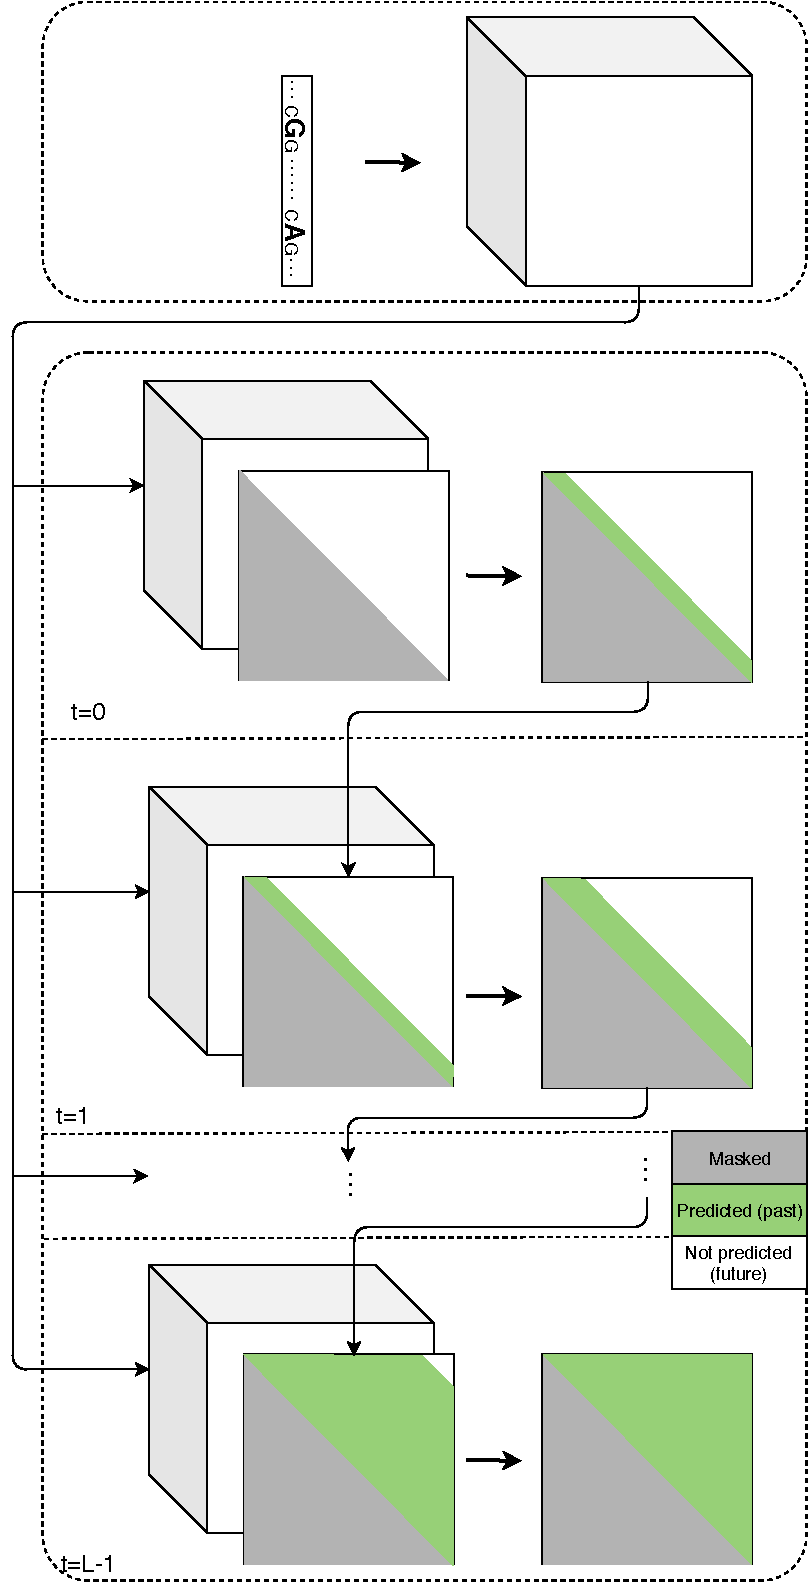
\includegraphics[width=0.35\textwidth]{plot/nn_arch_2.pdf}
        \caption{Sample structures conditioned on the input sequence.}
        \vspace{-3em}
        \label{fig:nn_arch_2}
        \centering
%    \end{figure}
\end{wrapfigure}


%TODO plot for NN architecture

%batch, mask

\subsection{Training}

We constructed a synthetic dataset for training the model, by sampling $50000$ random sequences.
For each sequence, the length is sampled uniformly from $10$ to $100$,
and each base is sampled \textit{i.i.d.} uniformly from $\{A, C, G, U\}$.
For each sequence, we ran RNAfold\cite{lorenz2011viennarna} with default parameters and
recorded the minimum free energy structure.

The model has $5$ pairs of 1D-conv layers, each having $256$ filters, with filter width and dilation rate being
$(7,1), (5,2), (5,2), (5,4), (5,4)$.
There are $5$ masked 2D-conv layers, each having $50$ filters, with filter size and dilation rate being
$([3,3],1), ([3,3],2), ([5,5],2), ([9,9],4), ([9,9],4)$.
Fully connected layer has $20$ hidden units. All layers use ReLU activation, except for the output layer being sigmoid.
$40000$ sequences were used for training and $10000$ for validation, with a batch size of $10$ sequences.
Adam optimizer\cite{kingma2014adam} was used with learning rate $0.001$
and the model was trained over $200$ epochs with early stopping.

%Number of layers, filter, dilation.
%minbatch size.
%Adam, learning rate.
%200 epochs with early stopping. $40000$ for training and $10000$ for validation.

For each batch, we zero-pad the sequence array and structure matrix to the maximum length in the batch.
When computing the loss and gradient,
both the lower triangular and the padding entries are masked.
%entries in structure matrix that were padded are masked,
%in addition to the lower triangular entries, since we're only predicting the upper triangular matrix.
At training time, prediction, loss, and gradient of all positions in the output are computed in parallel,
by passing in the target structure matrix as both the input and target.

%Note that although we present a single output structure for each input sequence at training time,
%the model is capable of generating a distribution of structures at test time, by generalizing across different examples.

%TODO hyperparameters

%Special constraints when sampling the matrix.

%Describe dataset.

%1-step AR.


\subsection{Inference} \label{sec:inference}

%TODO this is repeated from the model section, maybe combine?

At test time, we sample structures conditioned on the input sequence.
As shown in Fig \ref{fig:nn_arch_2}, we first pass the sequence through the
sequence encoder network to get the 2D feature map.
We then initialize the structure matrix with all zeros, concatenate it with the 2D feature map,
and sample one slice at a time until the upper triangular matrix is filled with sampled values.
At each step, we sample a binary label for each position in the current slice based on the
Bernoulli probability predicted by the model.
To ensure the sampled structure is valid, when sampling the label for location (i, j),
if the i-th or j-th position is already paired with another position (from samples in previous timestamps),
 we set $y_{i, j}$ to $0$ without sampling from the model output.
For a sequence of length $L$, we run $L-1$ steps sequentially.
%Note that multiple outputs can be sampled in parallel at test time.




\section{Result}

%TODO show some training performance. how?

\begin{wrapfigure}{R}
    \centering
    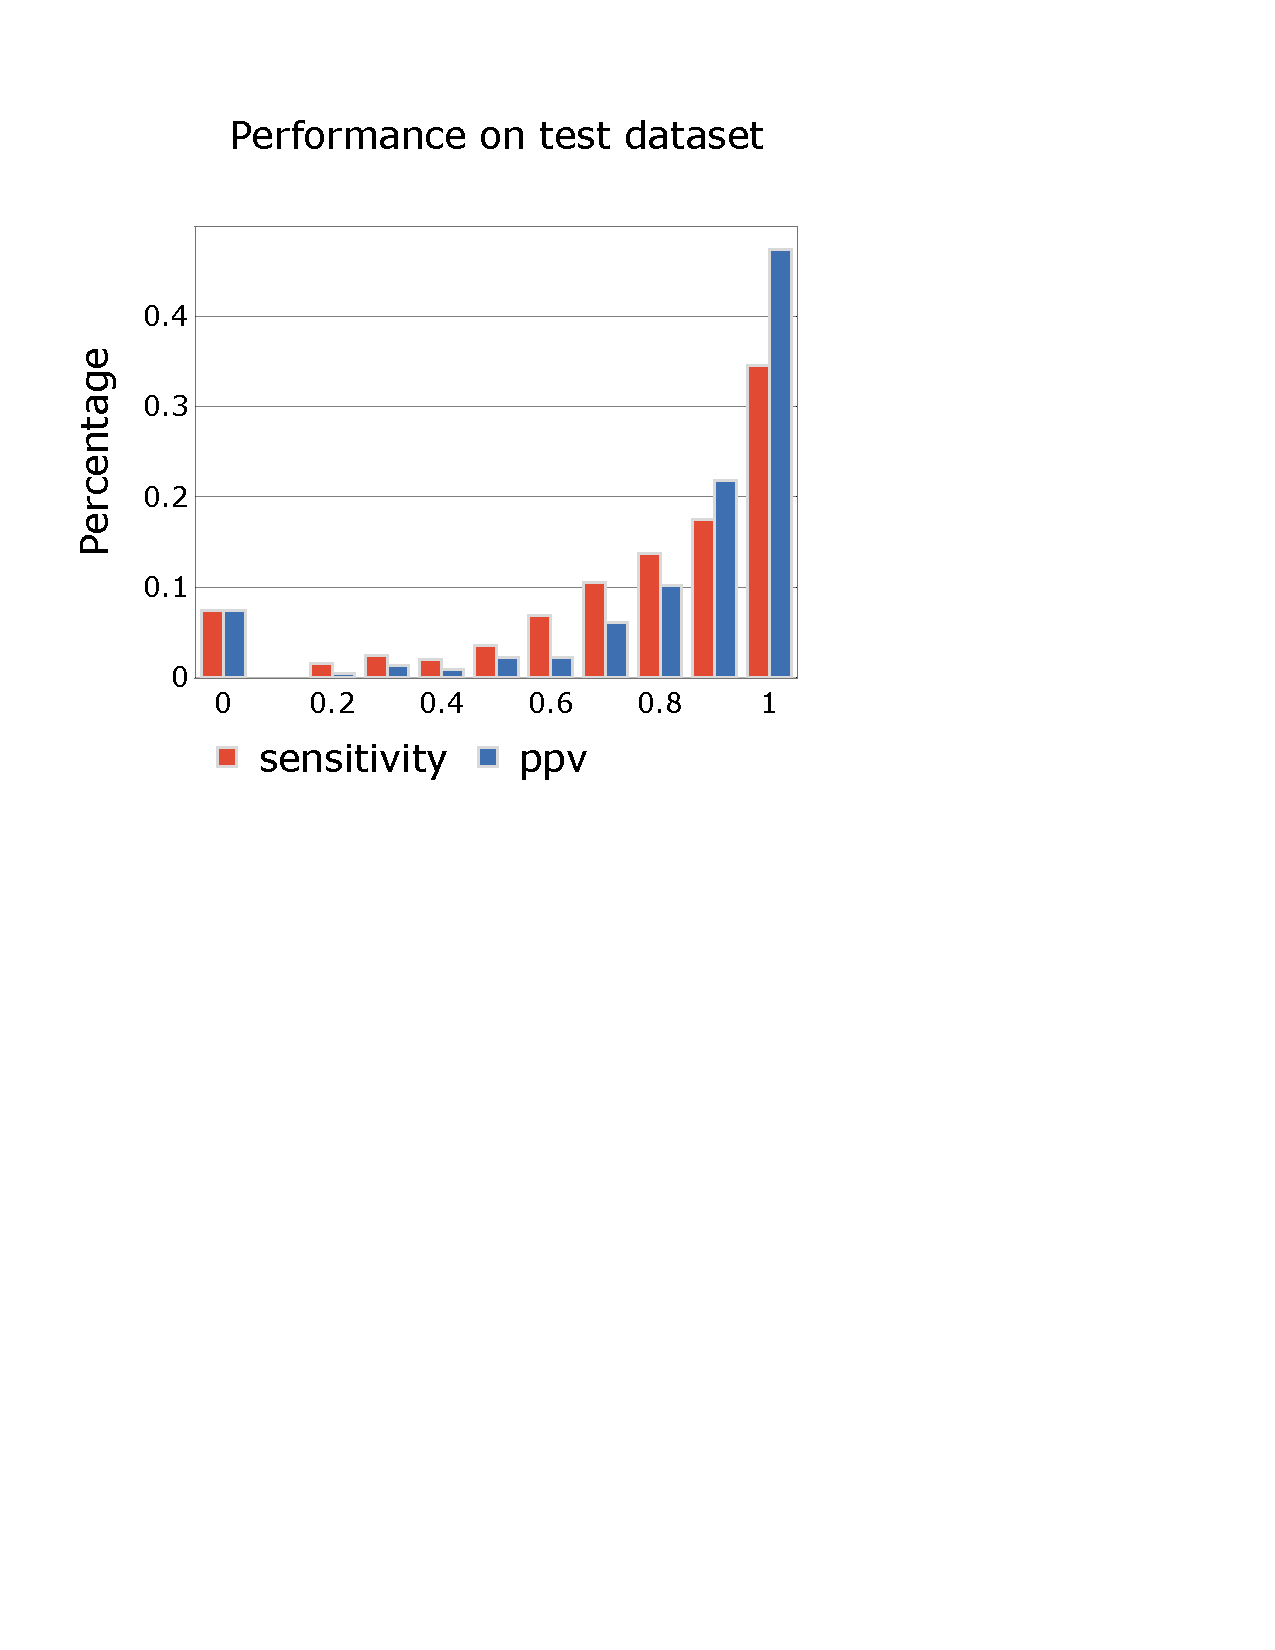
\includegraphics[width=0.3\textwidth]{plot/performance_test_set.pdf}
    \caption{Performance on test set.}
    \label{fig:performance_test_set}
    \centering
\end{wrapfigure}

\subsection{Test set performance}

To evaluate the model on unseen data, we generated a test set with $100$ sequence of length between $10$ and $100$,
using the same procedure that generated the training set.
%Sequences are generated with length between $10$ and $100$.
For each sequence in the test set, we ran RNAfold and sampled $100$ structures from the ensemble.
We also used our model to sample $100$ structures from the output distribution conditioned on each sequence.
To avoid evaluating on low probability samples, structures occurring only once were discarded.
To compare the two structure distributions,
for each unique structure produced by RNAfold, we computed sensitivity
(number of correctly predicted base pairs divided by number of true base pairs) and
positive predictive value (PPV, a.k.a. precision, number of correctly predicted base pairs
divided by number of predicted base pairs)
against all unique structures generated by our model
and recorded the best one, where best is defined by largest sensitivity + PPV.
This indicates how well the model recovers each of the structures produced by RNAfold.
Fig \ref{fig:performance_test_set} shows a the distribution of sensitivity and PPV across all structures in all sequences.
It can be observed that majority of the RNAfold-generated structures can be recovered with larger than $0.8$ sensitivity and PPV.




% TODO run RNAfold, generate top-n strutcures in ensembl
% TODO then sample e.g. 100 structures from our model, see how frequent we can recover the ones from RNAfold

%TODO show that we can predict well-known structure.
%Any known multi-structure sequences?

%\subsection{Generate distribution of structures}
%
%As an example, for a 323-base long sequence (TODO link to DB),
%we sampled 20 structure from the model output, as shown in Fig \ref{fig:sampled_structures}.
%On the left we show the binary upper triangular matrix sampled by the model (TODO it's too tiny to see anything),
%on the right we show the corresponding secondary structure rendered as a graph (only showing 4 due to space limit).
%
%
%\begin{figure}[h!]
%    \centering
%    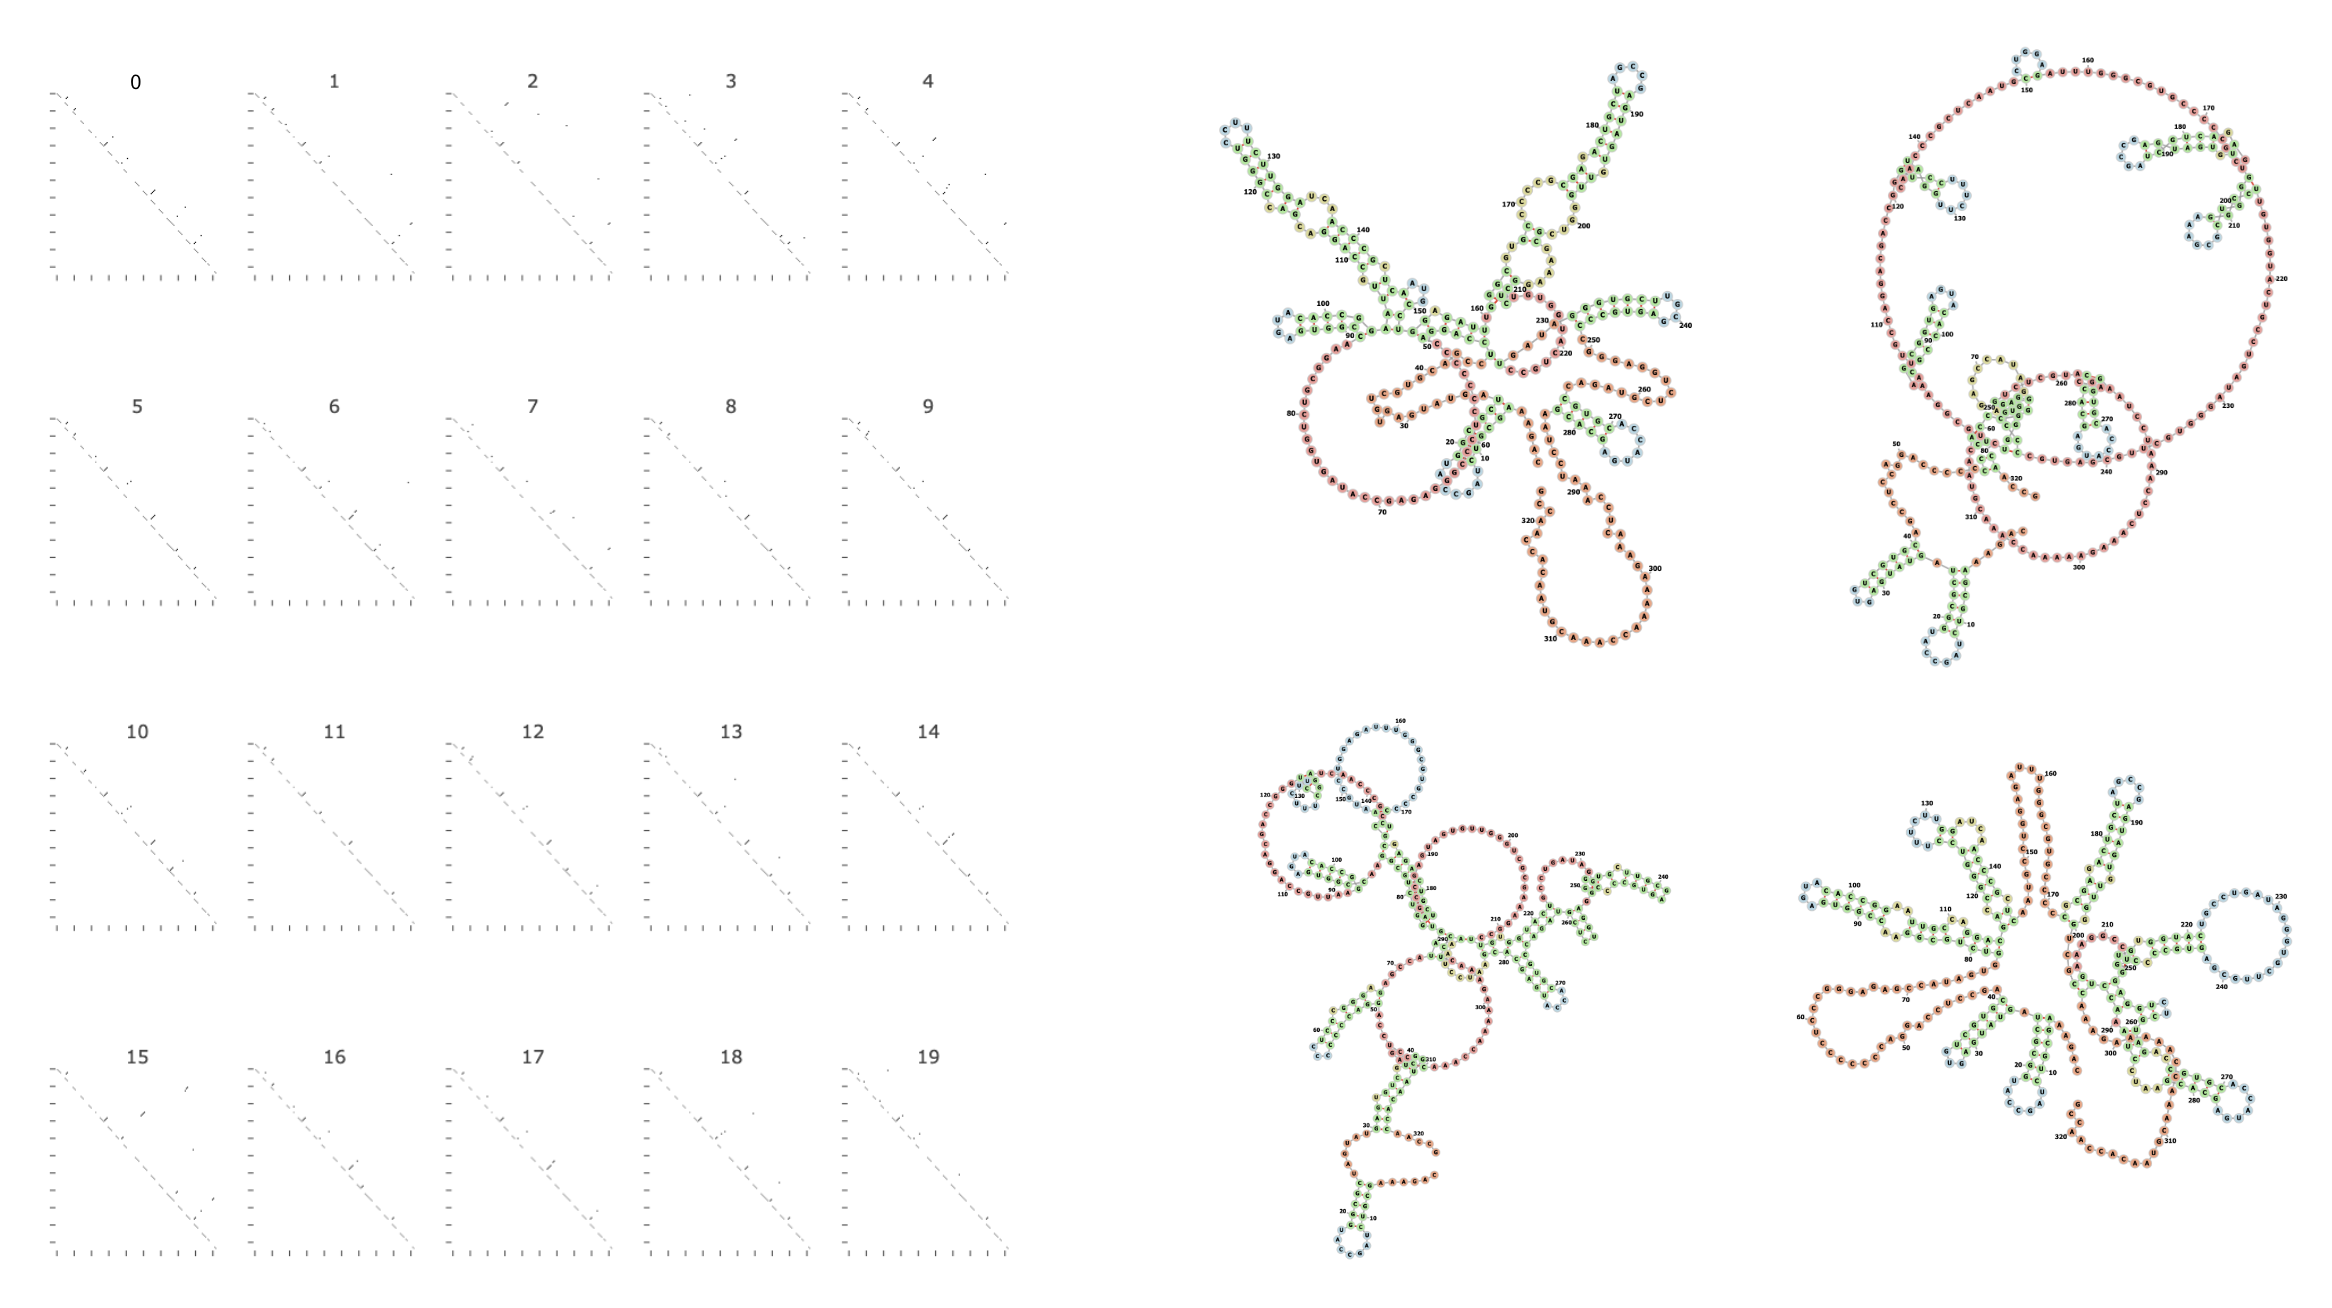
\includegraphics[width=\textwidth]{plot/sampled_structures.png}
%    \caption{TODO}
%    \label{fig:sampled_structures}
%    \centering
%\end{figure}


\begin{wrapfigure}{R}
    \centering
    \vspace{-3em}
    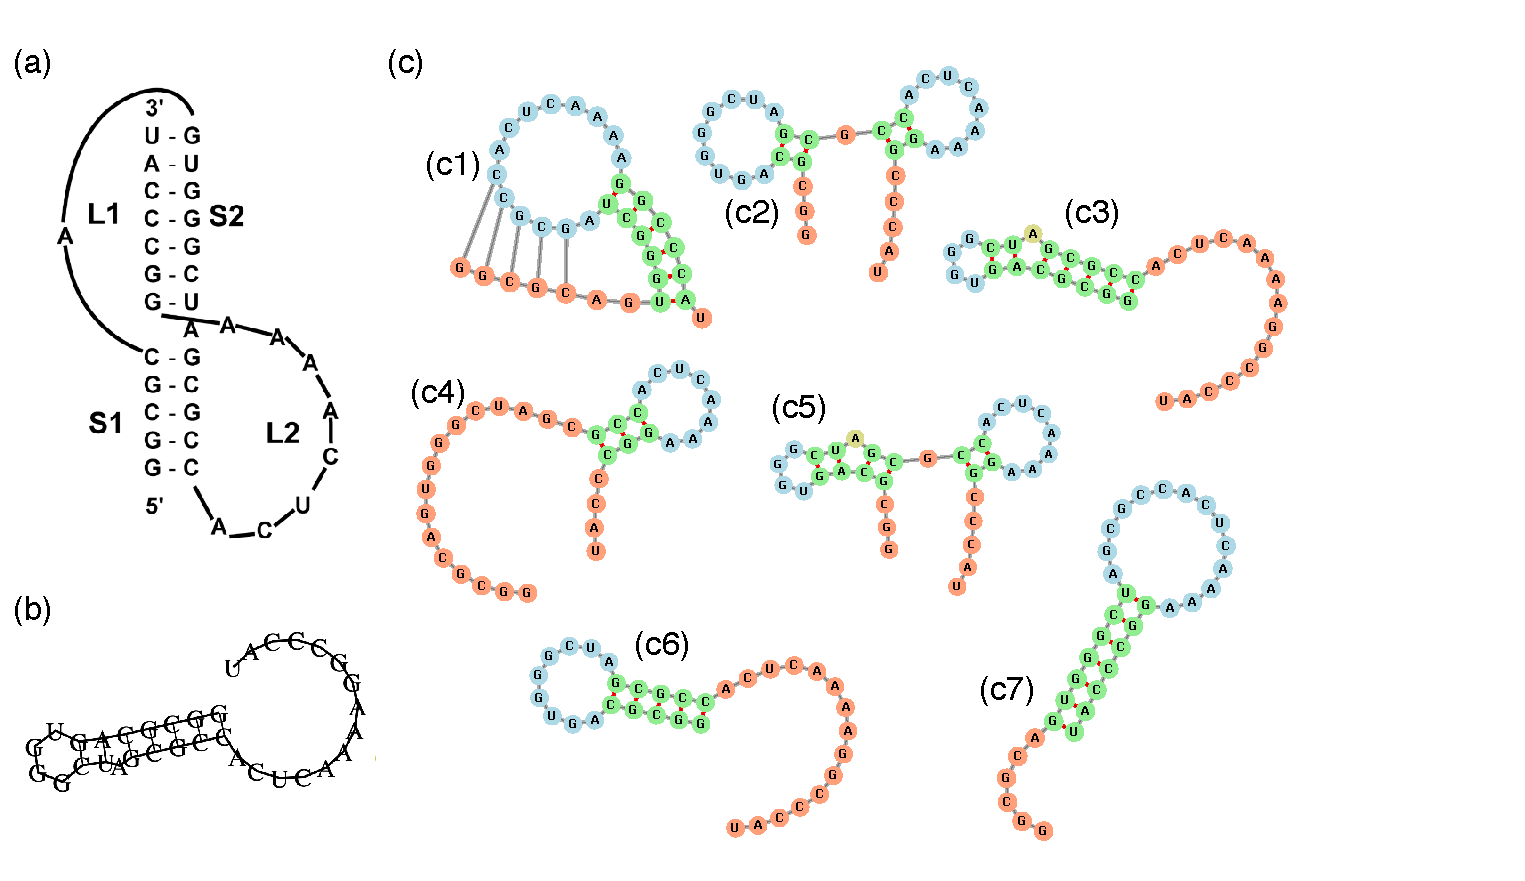
\includegraphics[width=0.5\textwidth]{plot/sample_structure_pseudoknot.pdf}
    \caption{Secondary structure of mouse mammary tumor virus (MMTV): (a) measured by nuclear magnetic resonance (NMR)\cite{staple2005pseudoknots}, (b) predicted by RNAfold, (c) generated by our model (only showing unique structures).}
    \vspace{-3em}
    \label{fig:sample_structure_pseudoknot}
    \centering
\end{wrapfigure}




%TODO show generating an ensemble of structures

\subsection{Structures with pesudoknot}

In addition to generating structures similar to the state-of-the-art models,
our model is also capable of predicting structures it has never seen during training,
since it does not incorporate hard-wired rules on how local structures assemble into global structure.
%Although trained on synthetic dataset with no pseudoknot structures,
%since our model doesn't incorporate hard-wired rules on how local structures assemble into global structure,
%it is actually capable of generating structure with pseudoknots.
As an example, we use the sequence of mouse mammary tumor virus (MMTV), whose secondary structure
contains pseudoknot as measured by nuclear magnetic resonance (NMR), as shown in Fig \ref{fig:sample_structure_pseudoknot}(a).
Minimum free energy structure predicted by RNAfold takes a quite different form, as shown in Fig \ref{fig:sample_structure_pseudoknot}(b).
In contrast, when we sampled $100$ structures from our model, we observed a diverse set of structures,
including the one predicted by RNAfold, as shown in Fig \ref{fig:sample_structure_pseudoknot}(c3),
and more interestingly, the pseudoknot structure from NMR, as shown in Fig \ref{fig:sample_structure_pseudoknot}(c1).

%and recovered ? with knots. (TODO also show other strutures? plot? pending fixing arr2db)
%See Fig \ref{fig:sample_structure_pseudoknot}.


%\subsection{Run time comparison}

%\subsection{Performance comparison}
%
%cross validation & test set (real sequences)
%
%\subsection{Interesting cases}

\subsection{Sequence design via gradient ascent}

One benefit of differentiable model is that we can answer interesting questions like:
given my current input sequence, what (small) changes can be made to maximize the pairing probability of two positions.
We illustrate this using a short RNA sequence GAUCACCUUUGGAUC.
The sequence is short enough such that vast majority of the structures in the distribution are identical,
as shown in Fig \ref{fig:gradient_ascent}(a).
We start with the current predicted structure and want to maximize base pairing at position $(i, j)$.
In order to find small changes to be made on this sequence,
we computed the gradient of the output node at $(i, j)$
with respect to all the input nodes ${\partial y_{i,j}}/{\partial \bm{x}}$.
We ran $100$ gradient ascent iterations with step size $0.01$.
In each step, after adding the gradient (times step size) onto the input,
we re-normalize the input so values along the feature dimension sum up to 1.
After all $100$ iterations, we convert the input matrix back to a sequence
by taking the nucleotide with max score for each position.
Fig \ref{fig:gradient_ascent}(b) and (c) shows the resulting sequence and structure
for $i=5, j=11$ and $i=6, j=10$, respectively.



\begin{wrapfigure}{l}
    \centering
    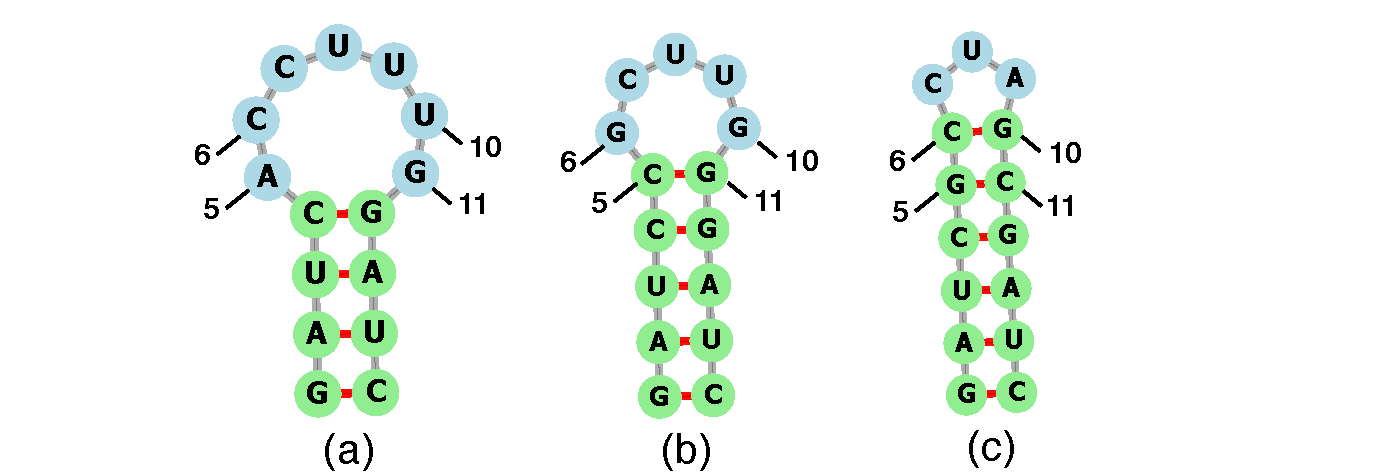
\includegraphics[width=0.25\textwidth]{plot/gradient_ascent.pdf}
    \caption{Sequence design via gradient ascent to maximize base pairing. (a) original structure, (b) maximize pairing at position (5, 11), (c) maximize pairing at position (6, 10).}
    \vspace{-8em}
    \label{fig:gradient_ascent}
    \centering
\end{wrapfigure}


%\begin{wrapfigure}{l}
%    \centering
%    \begin{minipage}[c]{0.25\textwidth}
%    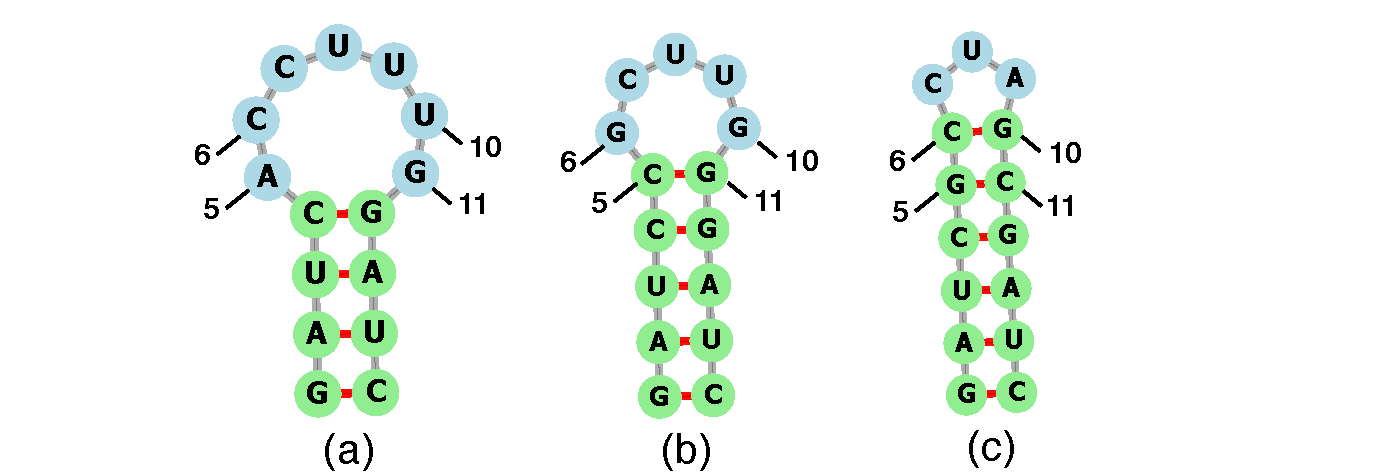
\includegraphics[width=0.25\textwidth]{plot/gradient_ascent.pdf}
%    \caption{Sequence design via gradient ascent to maximize base pairing. (a) original structure, (b) maximize pairing at position (5, 11), (c) maximize pairing at position (6, 10).}
%    \end{minipage}
%    \begin{minipage}[c]{0.2\textwidth}
%    \label{fig:gradient_ascent}
%\end{minipage}
%    \centering
%\end{wrapfigure}



%differentialble model. use case.

%\section{Conclusion}

%future work: train on real sequences and structure (we imagine the performance will improve)
%
%different AR/sampling setup, different factorization, better performance?
%
%train on high throughput data
%
%graph nn



\clearpage

\bibliographystyle{unsrt}
\bibliography{mlcb_2019}

%Speed consideration: implement split architecture, only need one forward pass for up to the last layer,
%then run last layer (triangular convolution) for $L-1$ times.
%
%
%Case study:
%
%TODO compare with RNAfold performance


\end{document}
